\documentclass{beamer}

\newcommand{\course}{CS 1331 Introduction to Object Oriented Programming}
\newcommand{\lesson}{Swing, Part 4 of 4}
\newcommand{\code}{http://www.cc.gatech.edu/~simpkins/teaching/gatech/cs1331/code}

\author[Chris Simpkins] 
{Christopher Simpkins \\\texttt{chris.simpkins@gatech.edu}}
\institute[Georgia Tech] % (optional, but mostly needed)

\date[CS 1331]{}


\newcommand{\course}{Introduction to Object-Oriented Programming}
\subject{\course}
\title[\lesson]{\course}
\subtitle{\lesson}

\author[CS 1331]
{Christopher Simpkins \\\texttt{chris.simpkins@gatech.edu}}
\institute[Georgia Tech]

\date[]{}

\newcommand{\link}[2]{\href{#1}{\textcolor{blue}{\underline{#2}}}}
\newcommand{\code}{http://cs1331.gatech.edu/code}

\usepackage{colortbl}

% If you have a file called "university-logo-filename.xxx", where xxx
% is a graphic format that can be processed by latex or pdflatex,
% resp., then you can add a logo as follows:

% \pgfdeclareimage[width=0.6in]{coc-logo}{cc_2012_logo}
% \logo{\pgfuseimage{coc-logo}}

\mode<presentation>
{
  \usetheme{Berlin}
  \useoutertheme{infolines}

  % or ...

 \setbeamercovered{transparent}
  % or whatever (possibly just delete it)
}

\usepackage{tikz}
% Optional PGF libraries
\usepackage{pgflibraryarrows}
\usepackage{pgflibrarysnakes}
\usepackage{pgfplots}
\usepackage{fancybox}
\usepackage{listings}
\usepackage{hyperref}
\hypersetup{colorlinks=true,urlcolor=blue}
\usepackage[english]{babel}
% or whatever

\usepackage[latin1]{inputenc}
% or whatever

\usepackage{times}
\usepackage[T1]{fontenc}
% Or whatever. Note that the encoding and the font should match. If T1
% does not look nice, try deleting the line with the fontenc.


\usepackage{listings}

% "define" Scala
\lstdefinelanguage{scala}{
  morekeywords={abstract,case,catch,class,def,%
    do,else,extends,false,final,finally,%
    for,if,implicit,import,match,mixin,%
    new,null,object,override,package,%
    private,protected,requires,return,sealed,%
    super,this,throw,trait,true,try,%
    type,val,var,while,with,yield},
  otherkeywords={=>,<-,<\%,<:,>:,\#,@},
  sensitive=true,
  morecomment=[l]{//},
  morecomment=[n]{/*}{*/},
  morestring=[b]",
  morestring=[b]',
  morestring=[b]""",
}

\usepackage{color}
\definecolor{dkgreen}{rgb}{0,0.6,0}
\definecolor{gray}{rgb}{0.5,0.5,0.5}
\definecolor{mauve}{rgb}{0.58,0,0.82}

% Default settings for code listings
\lstset{frame=tb,
  language=scala,
  aboveskip=2mm,
  belowskip=2mm,
  showstringspaces=false,
  columns=flexible,
  basicstyle={\scriptsize\ttfamily},
  numbers=none,
  numberstyle=\tiny\color{gray},
  keywordstyle=\color{blue},
  commentstyle=\color{dkgreen},
  stringstyle=\color{mauve},
  frame=single,
  breaklines=true,
  breakatwhitespace=true,
  keepspaces=true
  %tabsize=3
}


% If you wish to uncover everything in a step-wise fashion, uncomment
% the following command: 

% \beamerdefaultoverlayspecification{<+->}


\begin{document}

\begin{frame}
  \titlepage
\end{frame}

%------------------------------------------------------------------------
\begin{frame}[fragile]{WindowListeners, Adapters, Graphics and Drawing}


\begin{itemize}
\item {\tt WindowListener} and {\tt WindowAdapter}
\item {\tt ImageIcon}s
\item Graphics
\item Colors
\item Fonts and {\tt drawString}
\end{itemize}


\end{frame}
%------------------------------------------------------------------------

%------------------------------------------------------------------------
\begin{frame}[fragile]{{\tt java.awt.event.WindowListener}}


\begin{lstlisting}[language=Java]
public interface WindowListener extends EventListener {
    public void windowOpened(WindowEvent e);
    public void windowClosing(WindowEvent e);
    public void windowClosed(WindowEvent e);
    public void windowIconified(WindowEvent e);
    public void windowDeiconified(WindowEvent e);
    public void windowActivated(WindowEvent e);
    public void windowDeactivated(WindowEvent e);
}
\end{lstlisting}
See the API docs for details on each of these methods.
\begin{itemize}
\item To implement {\tt WindowListener}, you'd have to provide implementations for each method.
\item In most cases you're only interested in a few events.
\end{itemize}


\end{frame}
%------------------------------------------------------------------------

%------------------------------------------------------------------------
\begin{frame}[fragile]{{\tt java.awt.event.WindowAdapter}}


{\tt WindowAdapter} provides empty implementations of each method in {\tt WindowListener} (and a couple of other interfaces).
\begin{lstlisting}[language=Java]
public abstract class WindowAdapter
  implements WindowListener, WindowStateListener, WindowFocusListener {
    public void windowOpened(WindowEvent e) {}
    public void windowClosing(WindowEvent e) {}
    public void windowClosed(WindowEvent e) {}
    public void windowIconified(WindowEvent e) {}
    public void windowDeiconified(WindowEvent e) {}
    public void windowActivated(WindowEvent e) {}
    public void windowDeactivated(WindowEvent e) {}
    public void windowStateChanged(WindowEvent e) {}
    public void windowGainedFocus(WindowEvent e) {}
    public void windowLostFocus(WindowEvent e) {}
}
\end{lstlisting}
\vspace{-.1in}
\begin{itemize}
\item For simple window event listeners, extending {\tt WindowAdapter} is easier than implementing {\tt WindowListener}.
\item The standard library provides similar adapter classes for other large interfaces, such as {\tt MouseListener} ({\tt MouseAdapter}).
\end{itemize}


\end{frame}
%------------------------------------------------------------------------

%------------------------------------------------------------------------
\begin{frame}[fragile]{Using {\tt java.awt.event.WindowAdapter}}

\vspace{-.05in}
{\tt WindowAdapter} allows us to deal with only the single method from {\tt WindowListener} that we actually care about:
\vspace{-.05in}
\begin{lstlisting}[language=Java]
private class JackWindowListener extends WindowAdapter {
    public void windowClosing(WindowEvent e) {
        int choice = JOptionPane.showConfirmDialog(
            Jack.this,
            "Do you really want to exit?",
            "Exit for reals?",
            JOptionPane.OK_CANCEL_OPTION);
        if (choice == JOptionPane.YES_OPTION) {
            System.exit(0);
        }
    }
}
\end{lstlisting}
\vspace{-.05in}
Then you'd have the following lines in your constructor:
\vspace{-.05in}
\begin{lstlisting}[language=Java]
  // Need to set DO_NOTHING_ON_CLOSE so we can handle window closing
  setDefaultCloseOperation(DO_NOTHING_ON_CLOSE);
  
  // Confirm exit before exiting program
  addWindowListener(new JackWindowListener());
\end{lstlisting}

\end{frame}
%------------------------------------------------------------------------


%------------------------------------------------------------------------
\begin{frame}[fragile]{{\tt ImageIcon}s}


An {\it icon} is a fixed-sized picture.

\begin{itemize}
\item Swing components such as {\tt JButton}s, {\tt JMenuItem}s and {\tt JLabel}s can display {\tt ImageIcon}s.
\item Typical sizes for button and menu item icons are 16x16 or 32x32.  Oracle provides a set of ready-to-use icons in the \link{http://www.oracle.com/technetwork/java/index-138612.html}{Java look and feel Graphics Repository}
\item {\tt ImageIcon}s can be used for displaying any image, not just icons for GUI components. (But you wouldn't use {\tt ImageIcon} as the basis for an image-editing application.)
\end{itemize}

Create an {\tt ImageIcon} by passing the name of an image file to the constructor:
\begin{lstlisting}[language=Java]
ImageIcon jackIcon = new ImageIcon("JACK-HEARTS.png");
\end{lstlisting}

Take a look at \link{\code/swing/Jack.java}{Jack.java} for simple examples of using {\tt ImageIcon}s and {\tt WindowAdapter}.
\end{frame}
%------------------------------------------------------------------------

%------------------------------------------------------------------------
\begin{frame}[fragile]{The {\tt paint} Method}


All {\tt java.awt.Component}s have a {\tt paint} method which you can override to draw arbitrary graphics on the screen.  The general form of such an overriden {\tt paint} method, shown here with a {\tt JFrame} is:

\begin{lstlisting}[language=Java]
public class MyFrame extends JFrame {
    // ...
    public void paint(Graphics g) {
        super.paint(g);
        // Custom drawing commands here ...
    }
}
\end{lstlisting}
\vspace{-.05in}
A component's {\tt paint} is called whenever the component
\begin{itemize}
\item is first made visible on the screen,
\item is resized, or
\item has damage that needs to be repaired. (For example, something that previously obscured the component has moved, and a previously obscured portion of the component has become exposed).
\end{itemize}


\end{frame}
%------------------------------------------------------------------------

%------------------------------------------------------------------------
\begin{frame}[fragile]{The {\tt Graphics} Object}


The {\tt java.awt.Graphics} instance that's passed into the {\tt paint} method keeps track of where the component is on the screen and provides component-relative drawing methods to draw on the component as well as methods to set background color and more.\\

Here's a simple demonstration of several {\tt Graphics} methods.  What does this paint?
\begin{lstlisting}[language=Java]
public void paint(Graphics g) {
    super.paint(g);
    g.setColor(new Color(207, 181, 59));
    g.drawArc(75, 50, 250, 200, 20, 340);
    g.drawLine(275, 150, 375, 150);
    g.drawLine(325, 150, 325, 250);
    g.setFont(new Font("Helvetica", Font.BOLD, 24));
    g.drawString("Go Tech!", 150, 275);
}
\end{lstlisting}

Try it out: \link{\code/swing/GtFrame.java}{GtFrame.java}

\end{frame}
%------------------------------------------------------------------------

%------------------------------------------------------------------------
\begin{frame}[fragile]{Coordinates on a {\tt Graphics} Object}


Here are the important points we used to draw the {\tt GtFrame}:
\vspace{-.1in}
\begin{center}
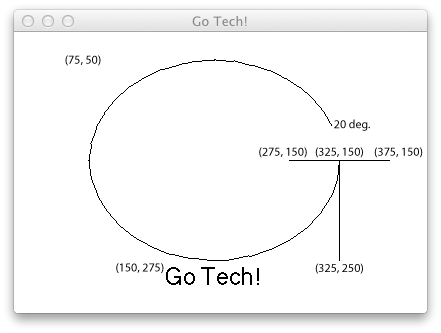
\includegraphics[height=2.2in]{gt-frame.png}
\end{center}
\vspace{-.2in}
Key points:
\begin{itemize}
\item (75, 50) is upper-left corner of the bounding rectangle for the arc.
\item {\tt drawArc} uses the 3-o'clock position as 0 degrees and sweeps counter-clockwise.
\end{itemize}


\end{frame}
%------------------------------------------------------------------------

%------------------------------------------------------------------------
\begin{frame}[fragile]{Closing Thoughts on Swing}


\begin{itemize}
\item There's much more to Swing and GUI programming.
\item You've learned the basics of GUIs and seen a good example of an object-oriented framework (Swing).
\item Underneath it all, it's just programs made of the same stuff we've learned already - data and processes, variables and control structures, classes and methods.
\item If you want to become a Java GUI programming ninja, learn JavaFX.  JavaFX is the future of GUI programming in Java.
\end{itemize}


\end{frame}
%------------------------------------------------------------------------



% %------------------------------------------------------------------------
% \begin{frame}[fragile]{}


% \begin{lstlisting}[language=Java]

% \end{lstlisting}

% \begin{itemize}
% \item
% \end{itemize}


% \end{frame}
% %------------------------------------------------------------------------


\end{document}
